\section{Durchführung}
\subsection{Theoretischer Teil}

\subsection{Kalibriermessungen}
    \subsubsection{Messung einer Quelle bekannter Aktivität bei mittiger Quellposition}
       Zunächst haben wir eine Quelle in mittigem Abstand zu den beiden Detektoren vermessen. Die Quelle hatte am 29.10.2015 eine Aktivitiät $A = \unit[1,02]{MBq}$.\\
       \vspace{2mm}
        
       \begin{tabular}{p{6cm}p{6cm}l}
               \minipanf 
                   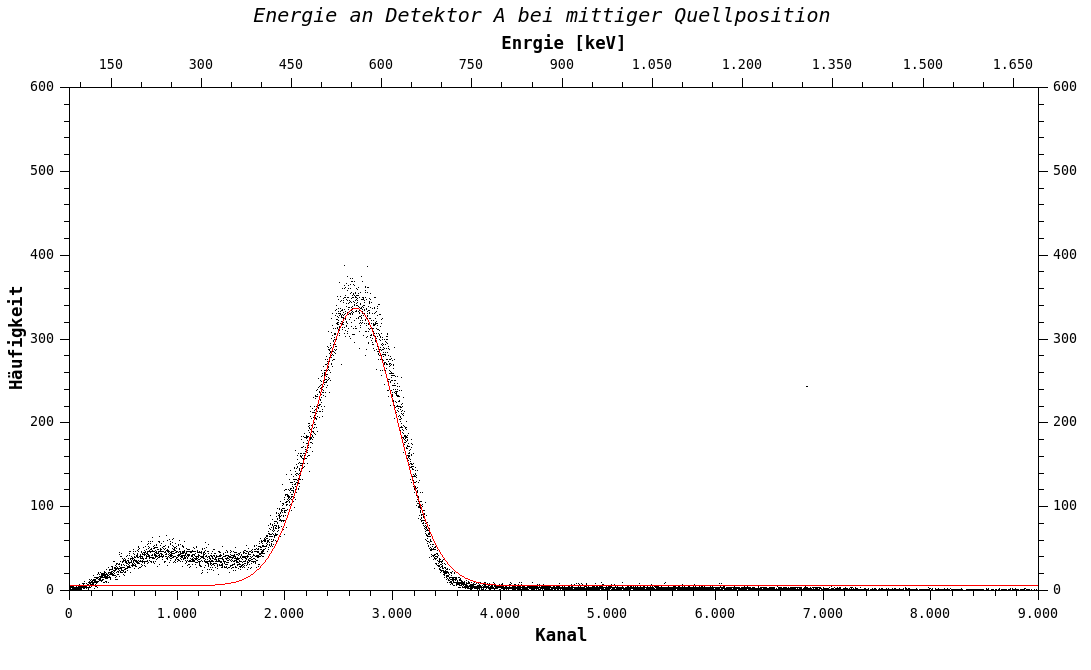
\includegraphics[width=1.2\textwidth, height=0.225\textheight]{pic/Efenster_DetA_M.png}
                   \label{dfd:EdetA_M}
               \minipend
               &
               \hspace{9mm}
               \minipanf 
                   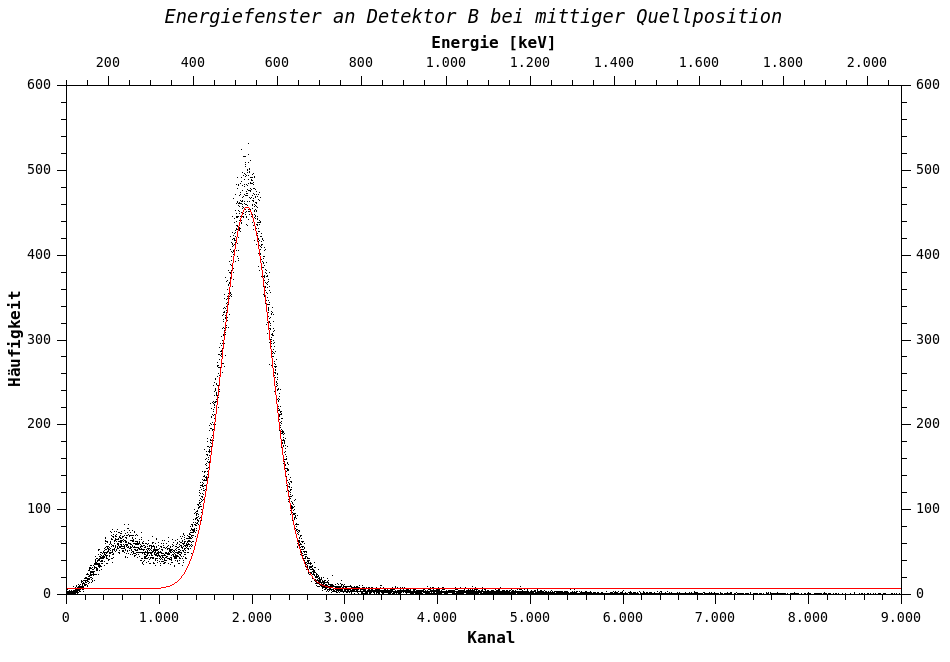
\includegraphics[width=1.2\textwidth, height=0.225\textheight]{pic/Efenster_DetB_M.png}
                   \label{dfd:EdetB_M}
               \minipend\\
               \multicolumn{2}{c}{\hspace{1.5cm}
                   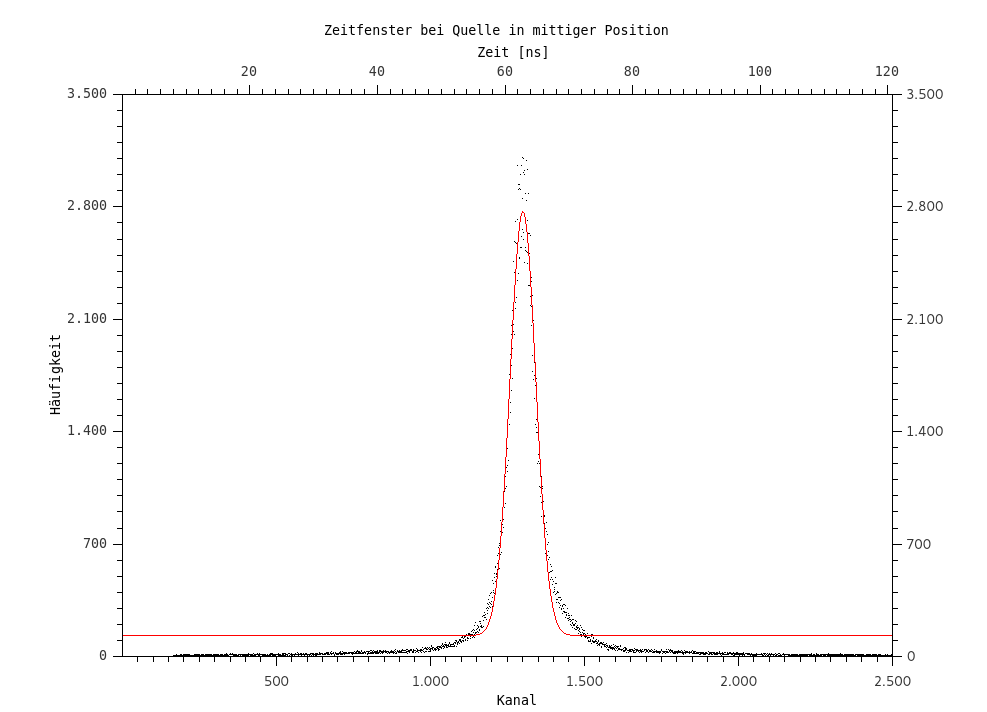
\includegraphics[width=0.7\textwidth, height=0.3\textheight]{pic/T_M_dia.png}
                   \label{dfd:T_M}}\\                        
       \end{tabular}
       \captionof{table}{Kalibrationsmessung bei Quelle mittig zwischen den Detektoren A und B}


    \subsubsection{Messung bei Positionen direkt an den Detektoren}
        \begin{tabular}{p{6cm}p{6cm}l}
            \minipanf 
                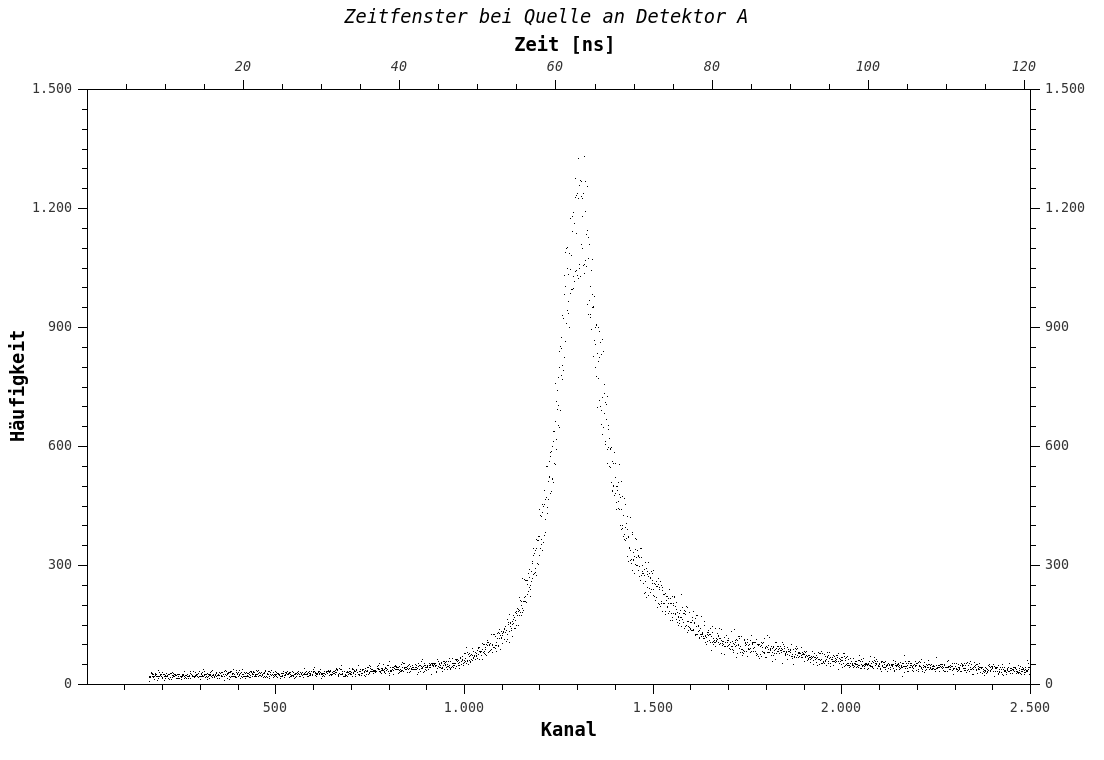
\includegraphics[width=1.2\textwidth, height=0.225\textheight]{pic/T_A_dia.png}
                \label{dfd:T_A}
            \minipend
            &
            \hspace{9mm} 
            \minipanf
                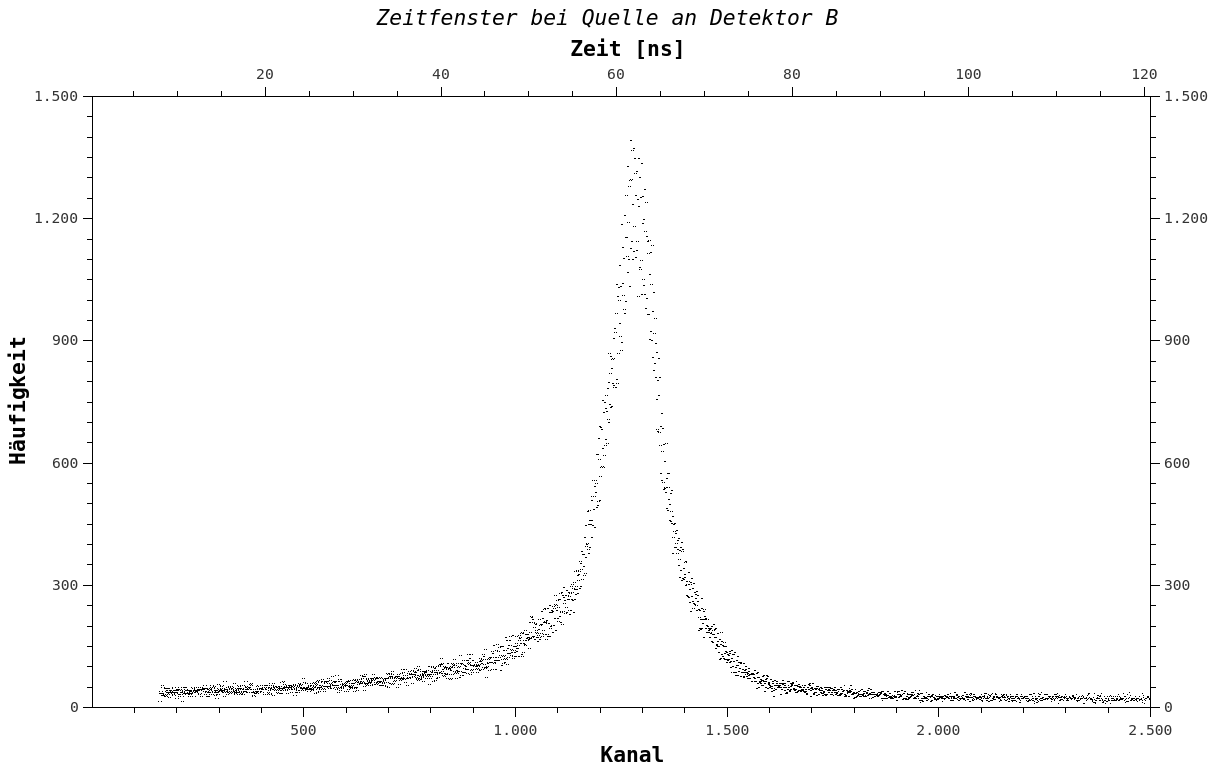
\includegraphics[width=1.2\textwidth, height=0.225\textheight]{pic/T_B_dia.png}
                \label{dfd:T_B}
            \minipend \\
            \minipanf
                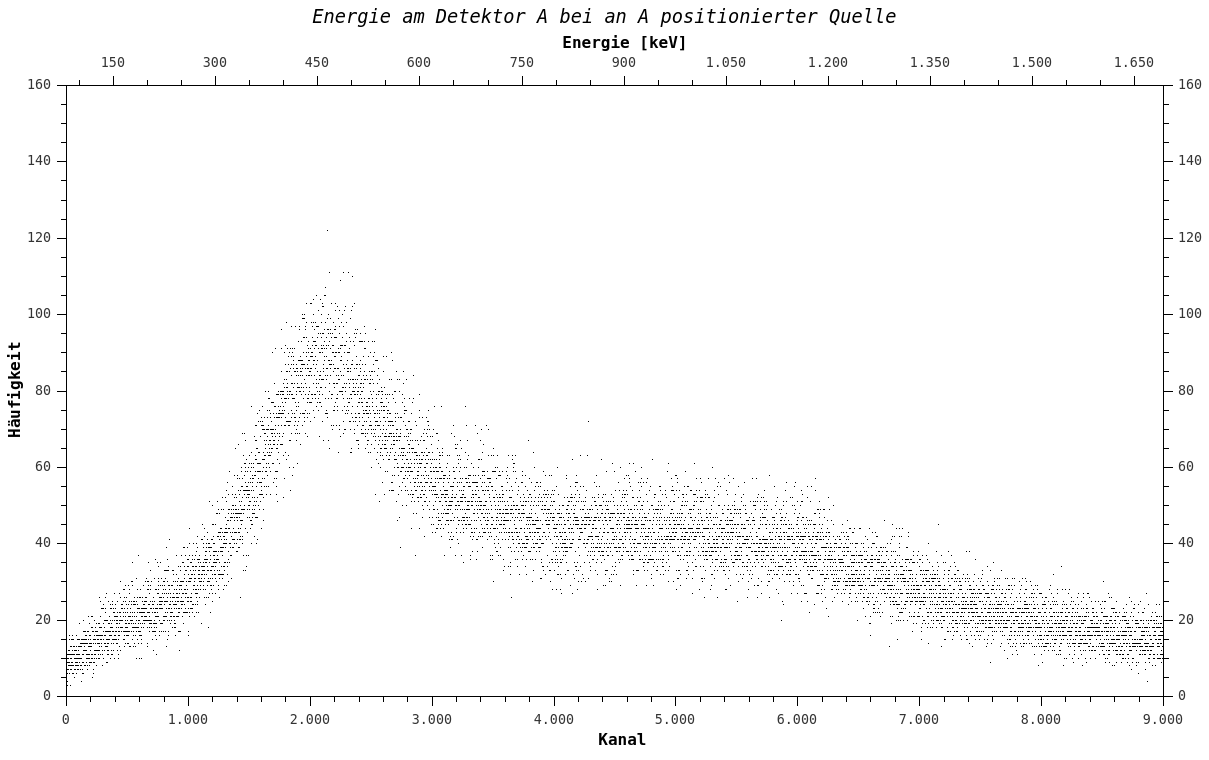
\includegraphics[width=1.2\textwidth, height=0.225\textheight]{pic/Efenster_DetA_A.png}
                \label{dfd:EdetAA}
            \minipend
            &
            \hspace{9mm} 
            \minipanf 
                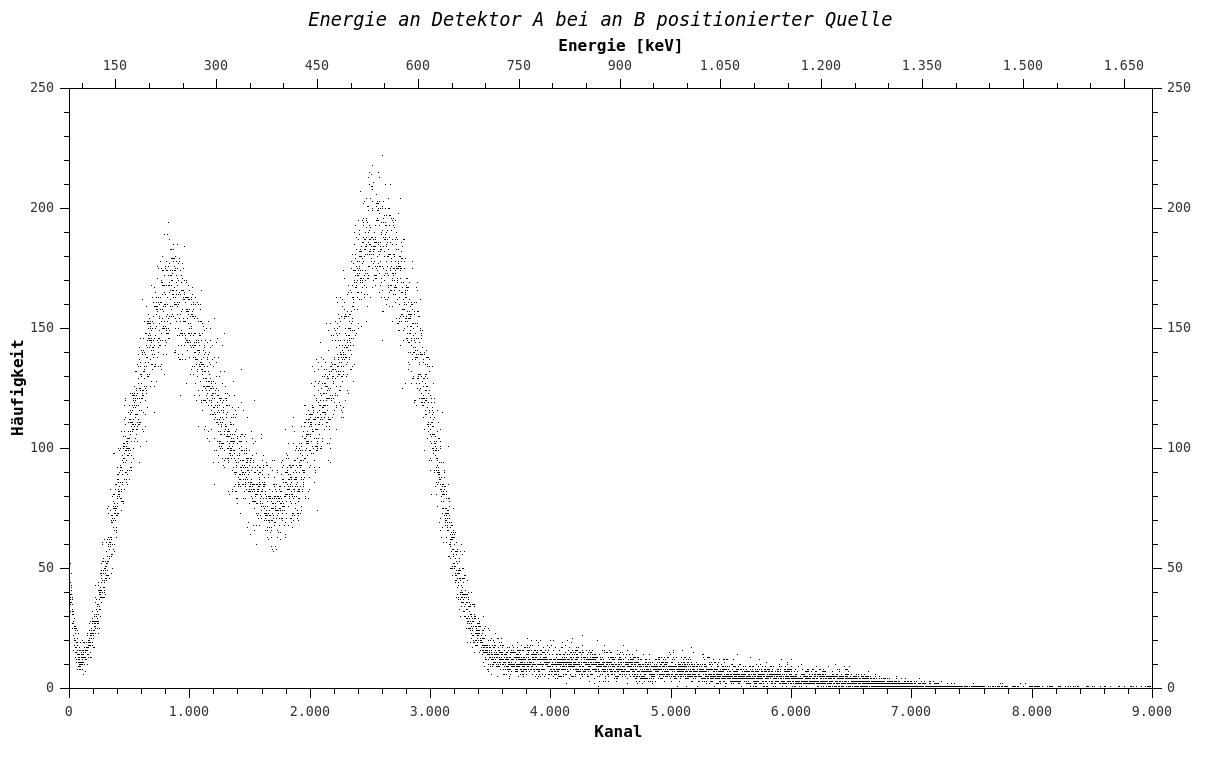
\includegraphics[width=1.2\textwidth, height=0.225\textheight]{pic/Efenster_DetA_B.png}
                \label{dfd:EdetBA}
            \minipend \\
            \minipanf 
                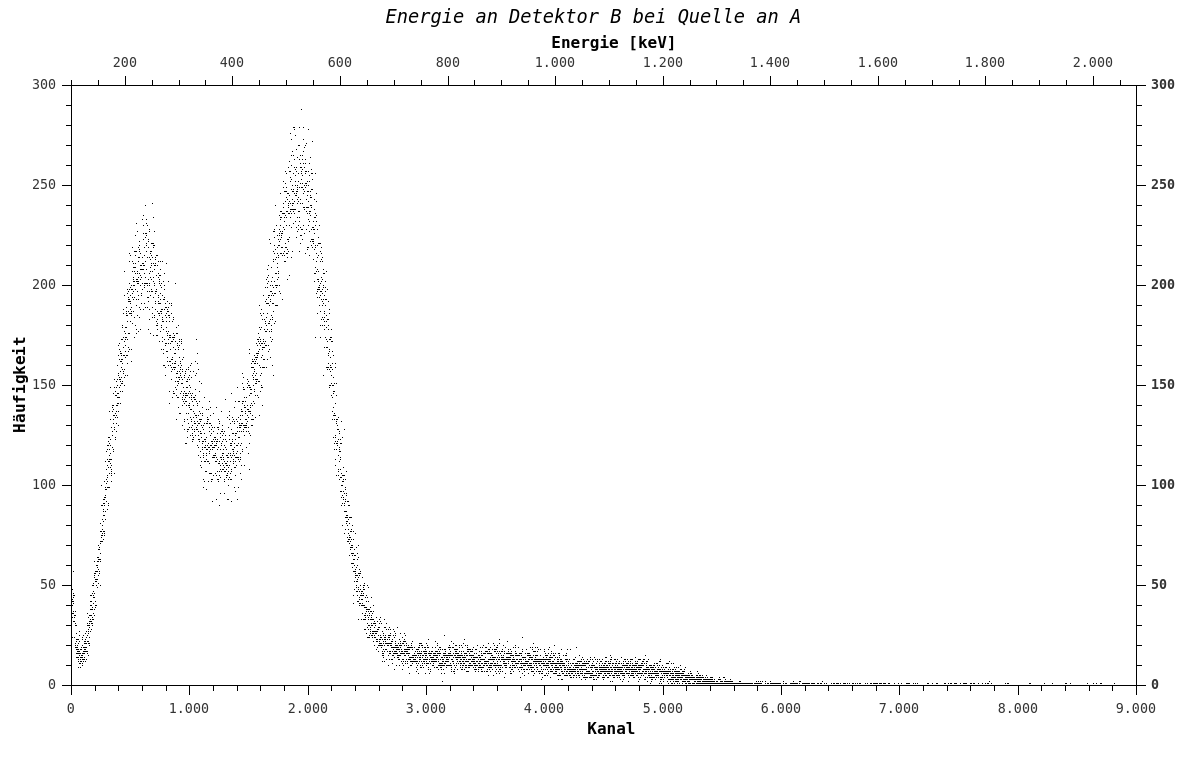
\includegraphics[width=1.2\textwidth, height=0.225\textheight]{pic/Efenster_DetB_A.png}
                \label{dfd:EdetAB}
            \minipend
            &
            \minipanf 
                \hspace{9mm}
                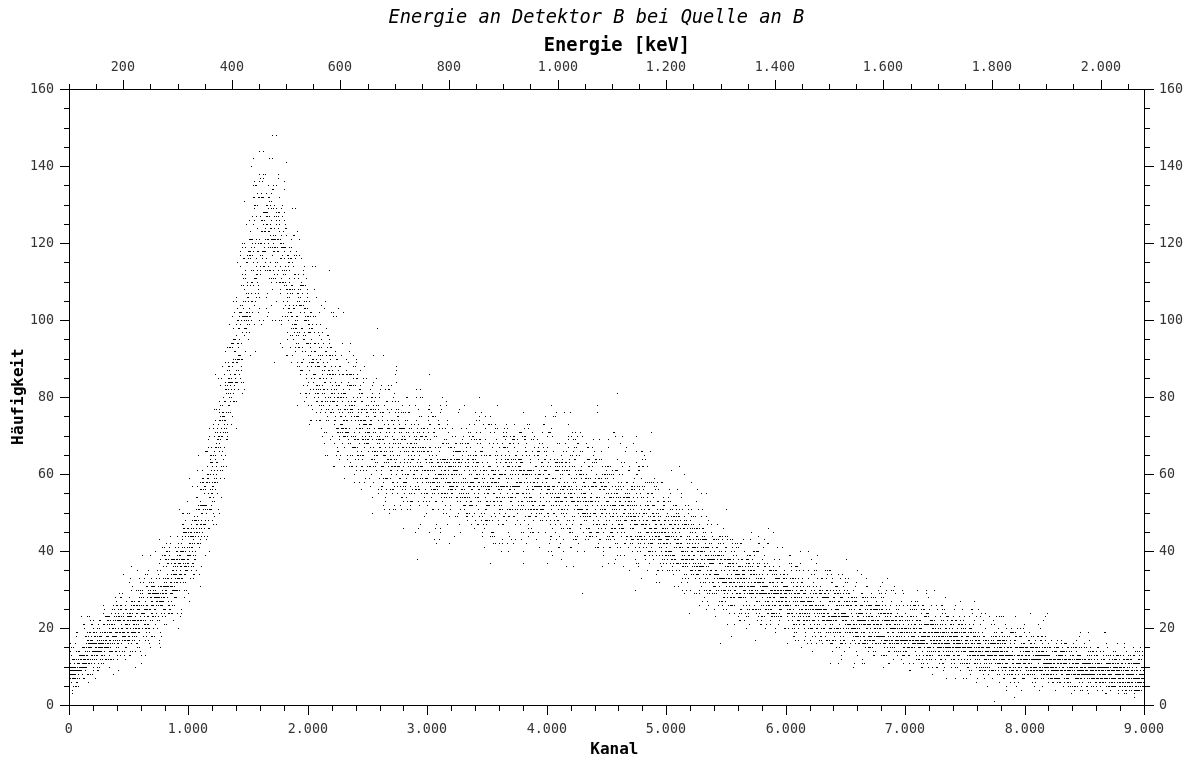
\includegraphics[width=1.2\textwidth, height=0.225\textheight]{pic/Efenster_DetB_B.png}
                \label{dfd:EdetBB}
            \minipend \\            
        \end{tabular}
        \captionof{figure}{Gegenüberstellung der Messungen mit der Quelle an Det. A (links) und Det. B (rechts)} 
        
    \subsection{Tomografische Messungen}
        \subsubsection{Messung einer Quellkonfiguration, Phantom isotroper Dichteverteilung}
          \textbf{Hauptversuch}\\
             \ \\
          Als nächsten wurde eine Messung mit unbekannter Quellverteilung gestartet. Die Energie- und das Zeitfenster entsprechen den oben bestimmten Intervallen.
          \minipanf  
            \begin{center}
            \begin{tabular}{p{7cm}p{7cm}c}
                ungefilterter Projektion & gefilterte Rückprpjektion\\
                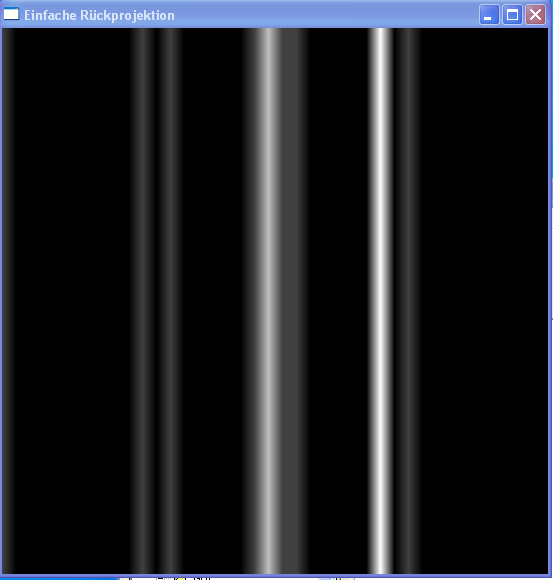
\includegraphics[width=0.3\textwidth, height=0.2\textheight]{pic/Einzelfenster_Bilder/unbekannte_Quelle/unbek1_einf_prj.png}
                & 
                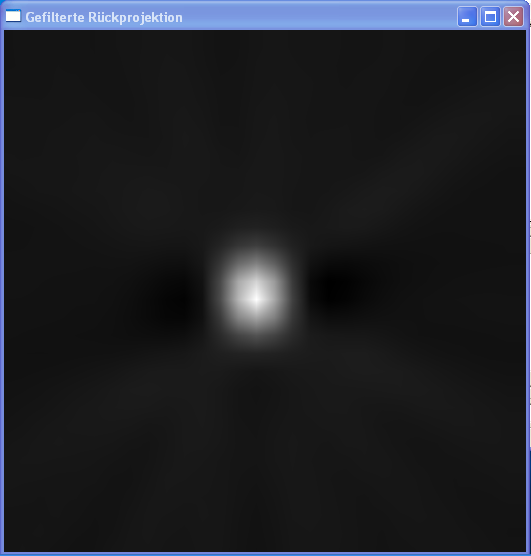
\includegraphics[width=.3\textwidth, height=0.2\textheight]{pic/Einzelfenster_Bilder/unbekannte_Quelle/unbek1gef_prj.png}\\
                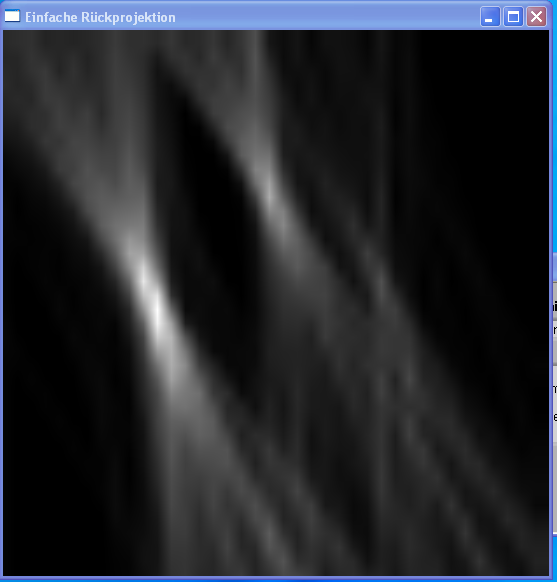
\includegraphics[width=0.3\textwidth, height=0.2\textheight]{pic/Einzelfenster_Bilder/unbekannte_Quelle/unbek2einf_prj.png}
                & 
                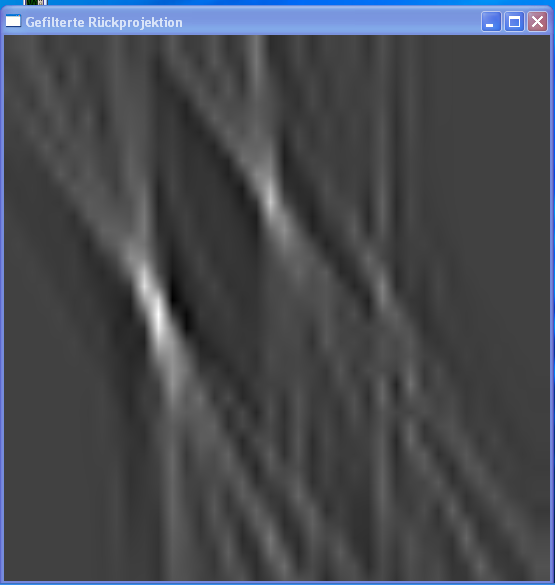
\includegraphics[width=.3\textwidth, height=0.2\textheight]{pic/Einzelfenster_Bilder/unbekannte_Quelle/unbek2gef_prj.png}\\ 
                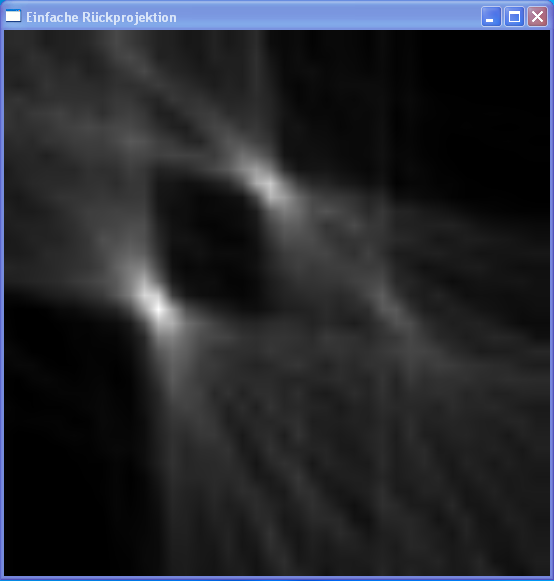
\includegraphics[width=0.3\textwidth, height=0.2\textheight]{pic/Einzelfenster_Bilder/unbekannte_Quelle/unbek3einf_prj.png}
                & 
                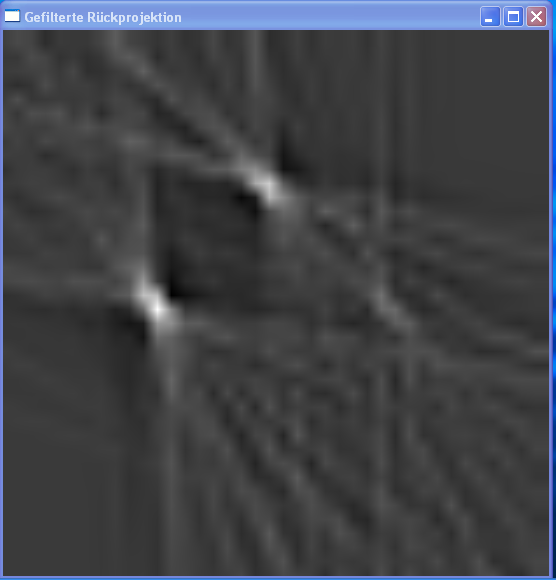
\includegraphics[width=.3\textwidth, height=0.2\textheight]{pic/Einzelfenster_Bilder/unbekannte_Quelle/unbek3gef_prj.png}\\               
                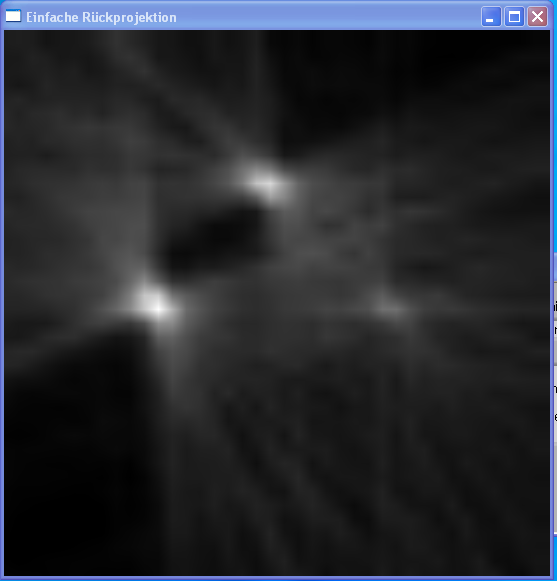
\includegraphics[width=0.3\textwidth, height=0.2\textheight]{pic/Einzelfenster_Bilder/unbekannte_Quelle/unbek4einf_prj.png}
                & 
                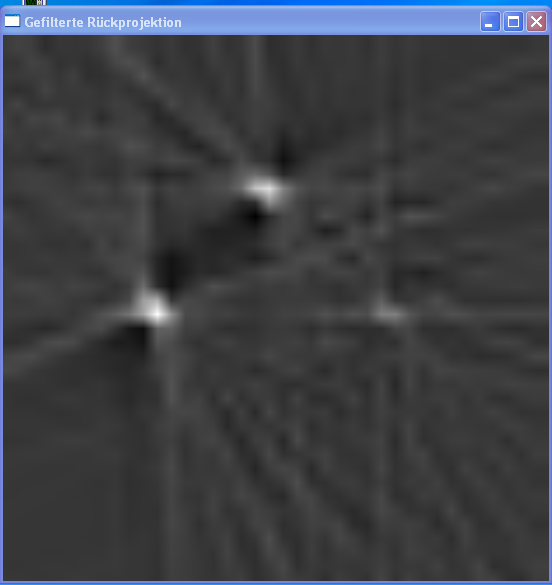
\includegraphics[width=.3\textwidth, height=0.2\textheight]{pic/Einzelfenster_Bilder/unbekannte_Quelle/unbek4gef_prj.png} \pagebreak
            \end{tabular}
            \end{center}
            \captionof{figure}{Screenshots der Bildenstehung der gefilterten (rechts) und ungefilterten (links) Rückprojektion}
          \minipend\\ \ \\
            \textbf{Untersuchung des Einflusses verschiedener Filter}\\
            
        \subsubsection{Messung mit einer Punktquelle, Phantom an-/insotroper Dichteverteilung}